\documentclass[10pt,twocolumn,letterpaper]{article}
\usepackage[T1]{fontenc}
\usepackage[review]{cvpr}
\usepackage{amsmath,amssymb,graphicx,booktabs}
\definecolor{cvprblue}{rgb}{0.21,0.49,0.74}
\usepackage[pagebackref,breaklinks,colorlinks,allcolors=cvprblue]{hyperref}
\def\paperID{*****}
\def\confName{CVPR}
\def\confYear{2027}
\newcommand{\method}{DecisionICL\xspace}
\title{DecisionICL\\Selecting Visual Demonstrations with Target-Model Decision Factors}
\author{Anonymous authors}
\begin{document}
\maketitlesupplementary
\renewcommand{\thesection}{\Alph{section}}
\renewcommand{\thetable}{S\arabic{table}}
\renewcommand{\thefigure}{S\arabic{figure}}

\section{Data and Implementation}
The supplementary material gives implementation details and complete results. A \emph{decision factor} describes a visual property through a set of states. A frozen encoder measures an image's \emph{factor evidence} against those state descriptions. A \emph{class prototype} averages training-image evidence within a labeled class. Retrieval class selection takes the highest fused score over these training classes. The resulting class index identifies the pool for demonstration retrieval. The target vision-language model (VLM) generates its final answer after receiving the retrieved demonstrations and query. A $k$-shot prompt contains $k$ labeled demonstrations. The ordered demonstrations for all queries form a retrieval plan.

In all tables, +D denotes the addition of \method. Differences are measured in percentage points (pp) and computed before rounding. CI denotes a confidence interval. SD denotes sample standard deviation across repeated runs. A rescue is correct only with the method named first in a comparison. A harm is correct only with its comparator. The difference $\Delta$ follows that orientation. Dataset and target names follow the main paper.

The experiments use the frozen partitions in Table~\ref{tab:splits}. The training split supplies the demonstration pool and class prototypes. Validation labels determine the base-factor mixture, with stratified five-fold out-of-fold evaluation followed by fitting on the complete validation split. Test labels are used to compute final metrics. The same partitions are shared across target models, retrieval methods, and demonstration budgets.

\begin{table*}[t]
\caption{Frozen dataset partitions after integrity and split-isolation checks. The demonstration budget refers to examples placed in the prompt. All methods have access to the complete labeled training pool.}
\label{tab:splits}
\centering
\begin{tabular}{lrrrr}
\toprule
Dataset & Classes & Train & Validation & Test \\
\midrule
DTD & 47 & 1,874 & 1,872 & 1,880 \\
FGVC-Aircraft & 100 & 3,334 & 3,333 & 3,333 \\
CUB-200-2011 & 200 & 5,993 & 1,000 & 4,794 \\
Stanford Dogs & 120 & 10,726 & 1,197 & 8,580 \\
Flowers 102 & 102 & 1,019 & 1,019 & 6,149 \\
\bottomrule
\end{tabular}
\end{table*}

\paragraph{Target models and inference.}
Qwen3-VL-4B-Instruct uses bfloat16 (BF16) precision. Qwen2.5-VL-7B-Instruct and Gemma 4 12B use 4-bit NormalFloat (NF4) double quantization with BF16 computation. Target generation is greedy with a maximum of 512 new tokens. Gemma's thinking mode is disabled, and its final content is extracted using the official response parser. An answer is correct only when its normalized text equals the class name. Other answers remain invalid and count as incorrect. Each target uses its own factor bank and generated CIRCLES descriptions.

\paragraph{Evidence and retrieval.}
RICES uses the frozen CLIP ViT-g/14 image representation. CLIP and SigLIP 2 are frozen image-text encoders. The classification-adapted MUIER uses SigLIP 2 image similarity plus query-image similarity to candidate class-name text, encoded as ``a photo of a $\{\text{class}\}$''. Factor measurement uses SigLIP 2 Base patch16 at resolution 224 and the template stated in the main paper. Native logits are normalized within each factor. Class prototypes are averages of training-image factor-state probabilities. For RICES and MUIER, the two selected demonstrations are distinct and ordered by base score. CIRCLES has an original-image ranking and a composed-description ranking, each called a retrieval channel. Its counterfactual description depicts an image after changing a visual attribute. Each channel selects its best example within the chosen class.

\begin{table*}[t]
\caption{Retained decision factors and states, reported as factors / states. These are the banks referenced by the accepted main-table plans. Discovery and filtering are performed on training material. Bank sizes reflect each target and dataset's frozen discovery protocol.}
\label{tab:banks}
\centering\small
\setlength{\tabcolsep}{9pt}
\begin{tabular}{lrrrrr}
\toprule
Target & DTD & Aircraft & CUB & Dogs & Flowers \\
\midrule
Qwen3-VL-4B & 36 / 107 & 29 / 81 & 11 / 33 & 35 / 125 & 108 / 304 \\
Qwen2.5-VL-7B & 93 / 303 & 80 / 260 & 92 / 342 & 79 / 279 & 100 / 373 \\
Gemma 4 12B & 74 / 183 & 73 / 201 & 77 / 210 & 82 / 250 & 68 / 208 \\
\bottomrule
\end{tabular}
\end{table*}

\section{Component and Source Controls}
\label{sec:source}
The controls use Qwen3-VL-4B with the same frozen data as the corresponding main results. Base-class selection is the no-factor ablation that uses the first RICES example to choose a class. It evaluates the complete DTD, Aircraft, and CUB test sets at two shots. It selects the class of the first RICES example, followed by the two highest-scoring images from that class's complete training pool. Its paired comparison with \method is reported below. Rescue and harm are oriented so that a rescue is correct only with \method.

\begin{table*}[t]
\caption{Paired results for \method compared with the base-class selection. Differences and intervals are percentage points. Exact $p$ values are raw two-sided McNemar values.}
\label{sup:gate_paired}
\centering\small
\begin{tabular}{lrrrrr}
\toprule
Dataset & Rescue & Harm & $\Delta$ (pp) & 95\% CI & Exact $p$ \\
\midrule
DTD & 68 & 33 & +1.862 & [0.798, 2.926] & 0.000641 \\
Aircraft & 429 & 124 & +9.151 & [7.831, 10.471] & 2.55e-40 \\
CUB & 133 & 72 & +1.272 & [0.688, 1.856] & 2.45e-05 \\
\bottomrule
\end{tabular}
\end{table*}

\paragraph{Prototype rotation and visual class centroids.}
The rotation control shifts prototype rows one position to the right in sorted class order and recalibrates the base mass independently. On CUB, calibration selects $\alpha=1$, so factor evidence has zero mass and retrieval follows base-class selection. A visual class centroid is the L2-normalized mean of a training class's unit CLIP image embeddings. The centroid control combines query-centroid cosine similarity with the original base-class score after standardizing both across classes. Its mixture receives independent validation calibration. Within-class retrieval and final VLM prompting remain unchanged. Table~\ref{sup:other_controls} reports the resulting final VLM accuracy. The centroid control exceeds \method by 5.05 pp on CUB, while the ordering reverses on Aircraft.

\begin{table*}[t]
\caption{Final VLM accuracy for additional class-evidence controls on Qwen3-VL-4B BF16 two-shot RICES. All variants retain within-class retrieval. The final column is control accuracy minus \method accuracy, calculated before rounding.}
\label{sup:other_controls}
\centering\small
\begin{tabular}{llrrr}
\toprule
Dataset & Control & Control acc. & DecisionICL & Control minus D \\
\midrule
DTD & Rotated prototypes & 76.70 & 78.78 & -2.07 \\
Aircraft & Rotated prototypes & 56.62 & 65.71 & -9.09 \\
CUB & Rotated prototypes & 79.50 & 80.77 & -1.27 \\
DTD & Visual class centroids & 79.20 & 78.78 & +0.43 \\
Aircraft & Visual class centroids & 63.82 & 65.71 & -1.89 \\
CUB & Visual class centroids & 85.82 & 80.77 & +5.05 \\
\bottomrule
\end{tabular}
\end{table*}

\paragraph{Matched factor sources.}
Decision discovery asks for task-discriminative visual properties. Generic discovery asks for general visual properties. The one-shot source experiment uses the same class-prototype retrieval architecture for both. Training-image inputs and request budgets are matched. The sources also share discovery perspectives and the structured response format. Only the discovery lead instruction changes. Each source variant receives an independent calibration for its base retriever. These controls use separate banks from the final main-table bank. Table~\ref{tab:source} gives all four accepted comparisons. Their differences vary in sign and magnitude.

\begin{table*}[t]
\caption{One-shot matched-source control. Decision and Generic accuracies use the same class-prototype architecture. The difference, rescue, and harm are oriented as Decision minus Generic.}
\label{tab:source}
\centering\small
\begin{tabular}{llrrrrrr}
\toprule
Dataset & Base & Decision & Generic & $\Delta$ & Rescue & Harm & Exact $p$ \\
\midrule
DTD & RICES & 76.596 & 76.968 & -0.372 & 30 & 37 & 0.464 \\
DTD & MUIER & 77.287 & 76.755 & +0.532 & 37 & 27 & 0.26 \\
Aircraft & RICES & 65.587 & 64.446 & +1.140 & 142 & 104 & 0.0181 \\
Aircraft & MUIER & 65.347 & 64.656 & +0.690 & 126 & 103 & 0.146 \\
\bottomrule
\end{tabular}
\end{table*}

\section{Class Selection and Final VLM Answers}
\label{sup:traces}
\paragraph{Frozen class readout.}
We compare the selected training class with the final VLM answer for Qwen3-VL-4B BF16 RICES+DecisionICL. This section uses the original seed-42 run, matching the main paper. Every demonstration in a context has the selected class as its training label. Reading that class from the frozen plan requires no additional VLM generation. Its accuracy is 78.67\% on DTD and 64.99\% on Aircraft. It is 81.29\% on CUB and 74.65\% on Dogs. Flowers 102 reaches 97.17\%. These readouts are identical across the two demonstration budgets.

At two shots, final-answer accuracy minus class-readout accuracy is $+0.11$ pp on DTD and $+0.72$ pp on Aircraft. It is $-0.52$ pp on CUB and $+3.59$ pp on Dogs. The difference on Flowers 102 is $+0.11$ pp. At one shot, the differences are $-1.12$ pp on DTD and $+0.39$ pp on Aircraft. They are $-5.90$ pp on CUB and $-0.28$ pp on Dogs. Flowers 102 gives $-4.02$ pp. On two-shot Dogs the VLM corrects 493 class-readout errors and introduces 185 errors. On two-shot CUB those counts are 38 and 63. This diagnostic scores the existing selection rule and its final answers without fitting another retrieval procedure. Appendix~\ref{sup:repeated} reports the separate repeated-run averages.

\paragraph{Score-to-context traces.}
The main-paper rescue and the failure below illustrate Qwen3-VL-4B two-shot RICES on Aircraft. We replay class selection for all 3,333 queries using the frozen retrieval inputs. These inputs contain factor evidence and training-class prototypes. They also bind CLIP similarities and the validation coefficients. All selected class indices match the accepted plans. Both methods' ordered demonstration identifiers also match. The final VLM answers are preserved from the accepted runs.

Let B be the class of the first RICES example and D the class selected by the combined score. Their score margin is
\begin{equation}
\begin{split}
m={}&\alpha(\widetilde b_D-\widetilde b_B)\\
&+\frac{1-\alpha}{G}\sum_{g=1}^{G}(\widetilde a_{g,D}-\widetilde a_{g,B}).
\end{split}
\end{equation}
The symbols $\widetilde b$ and $\widetilde a$ denote standardized base similarity and factor agreement. Both examples use $\alpha=0.20$ with $G=29$ factors. Each figure shows the query and each method's first retrieved training example. Image labels identify annotated training classes. The class-selection table reports the standardized scores and their fused value. A second table gives the measured state distributions for the largest positive individual factor contribution. The final-answer row reports VLM outputs generated after both demonstrations enter the context. These outputs are distinct from the class index used for retrieval.

\paragraph{Rescue trace.}
Query 2045488 is a Challenger 600. B denotes the first RICES demonstration's training class Embraer Legacy 600. D denotes the Challenger class chosen by retrieval class selection. Factor g10 describes the vertical stabilizer, which is the upright tail fin. Its states are tapered, rectangular, and rounded. Query evidence is $[0.015,0.228,0.757]$. The Legacy prototype is $[0.359,0.116,0.526]$. The Challenger prototype is $[0.026,0.265,0.709]$. These values measure relative whole-image compatibility with the descriptions. The weighted base term contributes $-0.040$ to the D-minus-B score margin. All factors together contribute $+0.944$. Their total margin of $+0.904$ selects the Challenger training class. Its retrieved demonstrations enter the VLM context. The final VLM answer is Challenger 600. With the RICES context the final answer is A319.

\paragraph{Failure trace.}
Query 0677579 contains several aircraft and has the ground-truth label DC-10. Its first RICES training example belongs to DC-10. The final VLM answer under RICES is also DC-10. Factor evidence shifts retrieval class selection to 747-100. The weighted factor margin is $+0.526$ and the base term is $-0.074$. Their sum is $+0.452$. The selected training class supplies two 747-100 demonstrations. After receiving this context the VLM generates the final answer 737-300. The selected training class and the final VLM answer therefore have different roles in the failure trace.

\begin{figure*}[t]
\centering
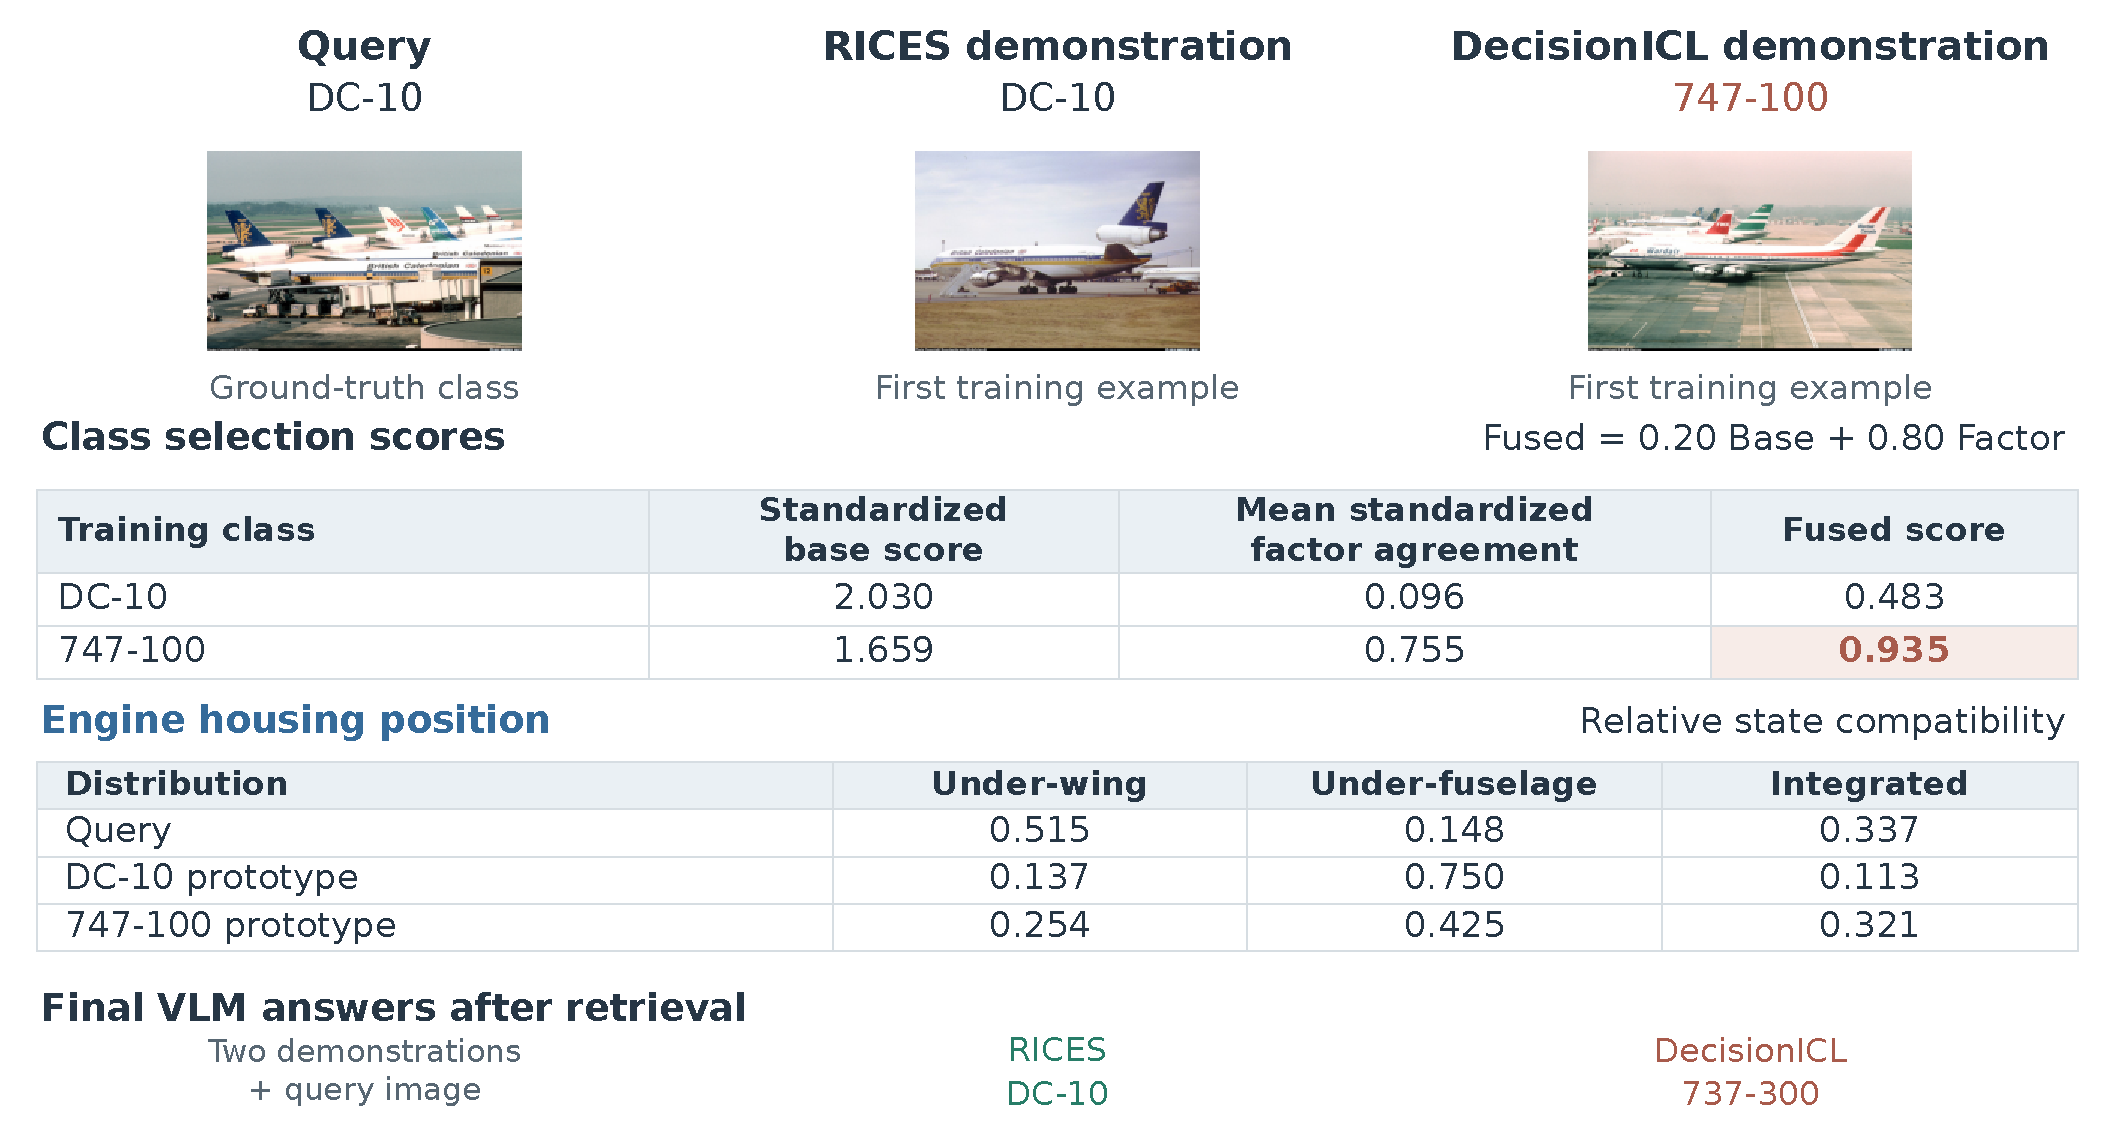
\includegraphics[width=\textwidth]{figures/algorithm_failure.pdf}
\caption{A failure that separates retrieval class selection from the final VLM answer. The query's ground-truth class is DC-10. The fused-score argmax selects the 747-100 training class. Its two retrieved demonstrations enter the context before the VLM generates the incorrect final answer 737-300. The displayed engine-housing-position factor gives the largest positive individual contribution to this class-selection score margin. The factor bank calls this property nacelle configuration.}
\label{fig:failure}
\end{figure*}

\paragraph{Example selection.}
For each outcome type, we consider test queries with different selected classes under the base and combined scores. We choose the query with the largest combined D-minus-B margin and break ties by sorted query identifier. Rescue and harm refer to final VLM answers. This rule selects explanatory high-margin cases after evaluation. The main paired results use every test query, and the examples make no claim about outcome frequency. Factor labels and measured values are unchanged. Only the figure's explanatory layout is new.

\section{Complete Main Accuracy Tables}
Tables~\ref{sup:full_main_0}, \ref{sup:full_main_1}, and~\ref{sup:full_main_2} report target-model accuracy in percent for the original seed-42 evaluation. The method suffix +D denotes \method. The one-shot setting has five methods and the two-shot setting has seven, giving 60 method results per target and 180 across the three targets.

\begin{table*}[t]
\caption{Qwen3-VL-4B BF16.}
\label{sup:full_main_0}
\centering\small
\begin{tabular}{llrrrrr}
\toprule
$k$ & Method & DTD & Aircraft & CUB & Dogs & Flowers \\
\midrule
1 & Random & 48.94 & 21.90 & 24.30 & 46.61 & 51.91 \\
1 & RICES & 76.06 & 56.62 & 74.30 & 72.74 & 92.75 \\
1 & RICES+D & 77.55 & 65.38 & 75.39 & 74.37 & 93.15 \\
1 & MUIER & 76.28 & 61.45 & 71.01 & 76.48 & 90.96 \\
1 & MUIER+D & 77.55 & 64.75 & 71.90 & 76.77 & 92.75 \\
2 & Random & 50.27 & 22.92 & 25.11 & 46.79 & 52.55 \\
2 & RICES & 77.87 & 59.20 & 79.10 & 77.41 & 97.25 \\
2 & RICES+D & 78.78 & 65.71 & 80.77 & 78.24 & 97.28 \\
2 & MUIER & 78.40 & 62.77 & 75.51 & 81.42 & 94.16 \\
2 & MUIER+D & 79.04 & 65.26 & 76.43 & 81.56 & 96.67 \\
2 & CIRCLES & 77.18 & 57.10 & 75.62 & 74.15 & 94.55 \\
2 & CIRCLES+D & 78.99 & 65.56 & 77.05 & 74.94 & 96.05 \\
\bottomrule
\end{tabular}
\end{table*}
\begin{table*}[t]
\caption{Qwen2.5-VL-7B NF4.}
\label{sup:full_main_1}
\centering\small
\begin{tabular}{llrrrrr}
\toprule
$k$ & Method & DTD & Aircraft & CUB & Dogs & Flowers \\
\midrule
1 & Random & 35.00 & 31.98 & 24.34 & 36.27 & 49.44 \\
1 & RICES & 65.05 & 51.37 & 70.34 & 68.66 & 94.41 \\
1 & RICES+D & 66.65 & 53.59 & 72.55 & 72.53 & 94.91 \\
1 & MUIER & 66.54 & 53.62 & 67.06 & 74.50 & 91.87 \\
1 & MUIER+D & 67.82 & 54.61 & 69.36 & 75.08 & 93.74 \\
2 & Random & 33.35 & 30.57 & 24.72 & 37.31 & 50.40 \\
2 & RICES & 66.86 & 57.16 & 75.64 & 72.49 & 97.11 \\
2 & RICES+D & 70.43 & 62.44 & 78.99 & 75.41 & 97.76 \\
2 & MUIER & 69.41 & 58.90 & 72.32 & 77.94 & 94.24 \\
2 & MUIER+D & 71.17 & 61.96 & 75.53 & 78.93 & 97.35 \\
2 & CIRCLES & 70.43 & 50.11 & 66.60 & 64.94 & 87.80 \\
2 & CIRCLES+D & 72.98 & 61.00 & 73.74 & 70.96 & 93.58 \\
\bottomrule
\end{tabular}
\end{table*}
\begin{table*}[t]
\caption{Gemma 4 12B NF4.}
\label{sup:full_main_2}
\centering\small
\begin{tabular}{llrrrrr}
\toprule
$k$ & Method & DTD & Aircraft & CUB & Dogs & Flowers \\
\midrule
1 & Random & 48.83 & 10.26 & 12.58 & 24.38 & 42.45 \\
1 & RICES & 72.18 & 51.49 & 73.61 & 62.31 & 90.89 \\
1 & RICES+D & 74.04 & 56.71 & 75.84 & 66.97 & 91.53 \\
1 & MUIER & 73.83 & 57.82 & 69.40 & 69.98 & 89.35 \\
1 & MUIER+D & 75.59 & 59.71 & 71.84 & 70.61 & 91.58 \\
2 & Random & 50.16 & 10.50 & 13.16 & 24.84 & 44.25 \\
2 & RICES & 73.09 & 52.03 & 74.43 & 66.83 & 94.88 \\
2 & RICES+D & 74.57 & 59.08 & 77.47 & 71.64 & 95.56 \\
2 & MUIER & 75.11 & 59.83 & 70.61 & 74.86 & 92.34 \\
2 & MUIER+D & 76.33 & 61.78 & 73.90 & 75.80 & 95.09 \\
2 & CIRCLES & 71.97 & 35.01 & 64.98 & 53.08 & 86.18 \\
2 & CIRCLES+D & 75.27 & 46.14 & 72.92 & 62.05 & 92.05 \\
\bottomrule
\end{tabular}
\end{table*}

\section{Paired Main Results}
Let $\hat y_P(q)$ denote the final VLM answer with the base context. Let $\hat y_D(q)$ denote its final answer with the \method context. These answers are generated after demonstration retrieval. Define $d_q=\mathbf{1}[\hat y_D(q)=y_q]-\mathbf{1}[\hat y_P(q)=y_q]$. A rescue has $d_q=1$ and a harm has $d_q=-1$. The accuracy difference is $100\sum_qd_q/n$ percentage points. Bootstrap intervals resample images with replacement 10,000 times using seed 42. The exact McNemar test conditions on the discordant pairs. Tables~\ref{sup:paired_0}, \ref{sup:paired_1}, and~\ref{sup:paired_2} contain individual comparison intervals and raw $p$ values.

\begin{table*}[t]
\caption{Qwen3-VL-4B BF16. All differences and intervals are in pp.}
\label{sup:paired_0}
\centering\small
\begin{tabular}{lllrrrrr}
\toprule
Dataset & $k$ & Base & $\Delta$ & Rescue & Harm & 95\% CI & Exact $p$ \\
\midrule
DTD & 1 & RICES & +1.489 & 54 & 26 & [0.585, 2.447] & 0.00232 \\
DTD & 1 & MUIER & +1.277 & 54 & 30 & [0.319, 2.234] & 0.0116 \\
Aircraft & 1 & RICES & +8.761 & 414 & 122 & [7.411, 10.081] & 3.73e-38 \\
Aircraft & 1 & MUIER & +3.300 & 172 & 62 & [2.430, 4.230] & 3.79e-13 \\
CUB & 1 & RICES & +1.085 & 108 & 56 & [0.563, 1.606] & 5.98e-05 \\
CUB & 1 & MUIER & +0.897 & 76 & 33 & [0.480, 1.335] & 4.66e-05 \\
Dogs & 1 & RICES & +1.632 & 339 & 199 & [1.107, 2.168] & 1.68e-09 \\
Dogs & 1 & MUIER & +0.291 & 44 & 19 & [0.117, 0.478] & 0.00223 \\
Flowers & 1 & RICES & +0.407 & 27 & 2 & [0.244, 0.569] & 1.62e-06 \\
Flowers & 1 & MUIER & +1.789 & 136 & 26 & [1.399, 2.195] & 3.51e-19 \\
DTD & 2 & RICES & +0.904 & 67 & 50 & [-0.213, 2.021] & 0.139 \\
DTD & 2 & MUIER & +0.638 & 60 & 48 & [-0.479, 1.702] & 0.29 \\
DTD & 2 & CIRCLES & +1.809 & 100 & 66 & [0.479, 3.138] & 0.0102 \\
Aircraft & 2 & RICES & +6.511 & 393 & 176 & [5.101, 7.891] & 4.79e-20 \\
Aircraft & 2 & MUIER & +2.490 & 192 & 109 & [1.470, 3.510] & 1.98e-06 \\
Aircraft & 2 & CIRCLES & +8.461 & 482 & 200 & [6.961, 9.961] & 9.14e-28 \\
CUB & 2 & RICES & +1.669 & 202 & 122 & [0.939, 2.399] & 1.03e-05 \\
CUB & 2 & MUIER & +0.918 & 152 & 108 & [0.271, 1.585] & 0.00754 \\
CUB & 2 & CIRCLES & +1.439 & 399 & 330 & [0.334, 2.524] & 0.0117 \\
Dogs & 2 & RICES & +0.828 & 487 & 416 & [0.140, 1.503] & 0.0198 \\
Dogs & 2 & MUIER & +0.140 & 199 & 187 & [-0.303, 0.594] & 0.576 \\
Dogs & 2 & CIRCLES & +0.793 & 581 & 513 & [0.035, 1.550] & 0.0428 \\
Flowers & 2 & RICES & +0.033 & 25 & 23 & [-0.179, 0.244] & 0.885 \\
Flowers & 2 & MUIER & +2.504 & 190 & 36 & [2.033, 2.992] & 1.8e-26 \\
Flowers & 2 & CIRCLES & +1.496 & 162 & 70 & [1.008, 1.984] & 1.42e-09 \\
\bottomrule
\end{tabular}
\end{table*}
\begin{table*}[t]
\caption{Qwen2.5-VL-7B NF4. Each row compares \method with its matching base on the same test queries.}
\label{sup:paired_1}
\centering\small
\begin{tabular}{lllrrrrr}
\toprule
Dataset & $k$ & Base & $\Delta$ & Rescue & Harm & 95\% CI & Exact $p$ \\
\midrule
DTD & 1 & RICES & +1.596 & 45 & 15 & [0.798, 2.394] & 0.000135 \\
DTD & 1 & MUIER & +1.277 & 35 & 11 & [0.585, 1.968] & 0.000536 \\
Aircraft & 1 & RICES & +2.220 & 183 & 109 & [1.230, 3.240] & 1.76e-05 \\
Aircraft & 1 & MUIER & +0.990 & 82 & 49 & [0.330, 1.680] & 0.00498 \\
CUB & 1 & RICES & +2.211 & 157 & 51 & [1.627, 2.795] & 9.46e-14 \\
CUB & 1 & MUIER & +2.295 & 231 & 121 & [1.523, 3.066] & 4.73e-09 \\
Dogs & 1 & RICES & +3.869 & 497 & 165 & [3.287, 4.464] & 1.52e-39 \\
Dogs & 1 & MUIER & +0.583 & 99 & 49 & [0.303, 0.862] & 4.83e-05 \\
Flowers & 1 & RICES & +0.504 & 41 & 10 & [0.276, 0.732] & 1.47e-05 \\
Flowers & 1 & MUIER & +1.870 & 141 & 26 & [1.480, 2.293] & 2.56e-20 \\
DTD & 2 & RICES & +3.564 & 106 & 39 & [2.340, 4.840] & 2.4e-08 \\
DTD & 2 & MUIER & +1.755 & 67 & 34 & [0.691, 2.819] & 0.00133 \\
DTD & 2 & CIRCLES & +2.553 & 108 & 60 & [1.223, 3.936] & 0.000264 \\
Aircraft & 2 & RICES & +5.281 & 371 & 195 & [3.870, 6.691] & 1.21e-13 \\
Aircraft & 2 & MUIER & +3.060 & 226 & 124 & [1.950, 4.140] & 5.45e-08 \\
Aircraft & 2 & CIRCLES & +10.891 & 556 & 193 & [9.301, 12.481] & 1.41e-41 \\
CUB & 2 & RICES & +3.358 & 319 & 158 & [2.461, 4.234] & 1.4e-13 \\
CUB & 2 & MUIER & +3.212 & 327 & 173 & [2.295, 4.110] & 5.33e-12 \\
CUB & 2 & CIRCLES & +7.134 & 613 & 271 & [5.945, 8.302] & 3.32e-31 \\
Dogs & 2 & RICES & +2.914 & 692 & 442 & [2.145, 3.683] & 1.14e-13 \\
Dogs & 2 & MUIER & +0.991 & 362 & 277 & [0.408, 1.562] & 0.000877 \\
Dogs & 2 & CIRCLES & +6.014 & 1056 & 540 & [5.117, 6.911] & 1.12e-38 \\
Flowers & 2 & RICES & +0.651 & 72 & 32 & [0.342, 0.976] & 0.00011 \\
Flowers & 2 & MUIER & +3.106 & 222 & 31 & [2.618, 3.627] & 9e-37 \\
Flowers & 2 & CIRCLES & +5.773 & 439 & 84 & [5.074, 6.489] & 5.31e-59 \\
\bottomrule
\end{tabular}
\end{table*}
\begin{table*}[t]
\caption{Gemma 4 12B NF4. Each row compares \method with its matching base on the same test queries.}
\label{sup:paired_2}
\centering\small
\begin{tabular}{lllrrrrr}
\toprule
Dataset & $k$ & Base & $\Delta$ & Rescue & Harm & 95\% CI & Exact $p$ \\
\midrule
DTD & 1 & RICES & +1.862 & 77 & 42 & [0.745, 2.980] & 0.00171 \\
DTD & 1 & MUIER & +1.755 & 85 & 52 & [0.532, 2.979] & 0.00605 \\
Aircraft & 1 & RICES & +5.221 & 319 & 145 & [3.960, 6.511] & 4.37e-16 \\
Aircraft & 1 & MUIER & +1.890 & 158 & 95 & [0.960, 2.850] & 8.98e-05 \\
CUB & 1 & RICES & +2.232 & 173 & 66 & [1.606, 2.858] & 3.05e-12 \\
CUB & 1 & MUIER & +2.441 & 205 & 88 & [1.752, 3.150] & 6.48e-12 \\
Dogs & 1 & RICES & +4.662 & 728 & 328 & [3.928, 5.408] & 1.76e-35 \\
Dogs & 1 & MUIER & +0.629 & 154 & 100 & [0.268, 1.002] & 0.000848 \\
Flowers & 1 & RICES & +0.634 & 53 & 14 & [0.374, 0.894] & 1.77e-06 \\
Flowers & 1 & MUIER & +2.228 & 153 & 16 & [1.837, 2.651] & 3.03e-29 \\
DTD & 2 & RICES & +1.489 & 98 & 70 & [0.160, 2.819] & 0.0369 \\
DTD & 2 & MUIER & +1.223 & 96 & 73 & [-0.108, 2.553] & 0.0903 \\
DTD & 2 & CIRCLES & +3.298 & 148 & 86 & [1.755, 4.894] & 6.09e-05 \\
Aircraft & 2 & RICES & +7.051 & 462 & 227 & [5.521, 8.611] & 2.2e-19 \\
Aircraft & 2 & MUIER & +1.950 & 253 & 188 & [0.720, 3.180] & 0.00227 \\
Aircraft & 2 & CIRCLES & +11.131 & 518 & 147 & [9.661, 12.601] & 2.45e-49 \\
CUB & 2 & RICES & +3.045 & 320 & 174 & [2.149, 3.942] & 5e-11 \\
CUB & 2 & MUIER & +3.296 & 301 & 143 & [2.441, 4.151] & 5.04e-14 \\
CUB & 2 & CIRCLES & +7.947 & 679 & 298 & [6.696, 9.220] & 7.2e-35 \\
Dogs & 2 & RICES & +4.814 & 921 & 508 & [3.963, 5.653] & 4.98e-28 \\
Dogs & 2 & MUIER & +0.944 & 340 & 259 & [0.385, 1.515] & 0.00106 \\
Dogs & 2 & CIRCLES & +8.974 & 1388 & 618 & [7.972, 9.977] & 9.63e-68 \\
Flowers & 2 & RICES & +0.683 & 90 & 48 & [0.309, 1.057] & 0.000441 \\
Flowers & 2 & MUIER & +2.748 & 198 & 29 & [2.277, 3.236] & 4e-32 \\
Flowers & 2 & CIRCLES & +5.871 & 521 & 160 & [5.058, 6.684] & 1.8e-45 \\
\bottomrule
\end{tabular}
\end{table*}

\section{Macro Accuracy and Invalid Outputs}
Tables~\ref{sup:macro_invalid_0}, \ref{sup:macro_invalid_1}, and~\ref{sup:macro_invalid_2} report macro accuracy in percent followed by the number of invalid class outputs. Macro accuracy averages the per-class accuracy. Invalid outputs are included as errors in both ordinary and macro accuracy. This preserves the original generation outcomes without output-format repair.

\begin{table*}[t]
\caption{Qwen3-VL-4B macro accuracy / invalid outputs.}
\label{sup:macro_invalid_0}
\centering\small
\begin{tabular}{llrrrrr}
\toprule
$k$ & Method & DTD & Aircraft & CUB & Dogs & Flowers \\
\midrule
1 & Random & 48.94 / 38 & 21.88 / 162 & 24.09 / 237 & 44.93 / 992 & 43.06 / 815 \\
1 & RICES & 76.06 / 11 & 56.63 / 37 & 74.60 / 38 & 71.74 / 319 & 91.35 / 207 \\
1 & RICES+D & 77.55 / 8 & 65.40 / 29 & 75.71 / 34 & 73.31 / 281 & 91.67 / 197 \\
1 & MUIER & 76.28 / 4 & 61.49 / 33 & 71.25 / 35 & 75.66 / 228 & 89.60 / 212 \\
1 & MUIER+D & 77.55 / 4 & 64.78 / 27 & 72.16 / 37 & 75.97 / 220 & 91.20 / 200 \\
2 & Random & 50.27 / 33 & 22.90 / 125 & 24.85 / 249 & 45.23 / 992 & 43.96 / 788 \\
2 & RICES & 77.87 / 8 & 59.20 / 26 & 79.30 / 18 & 76.56 / 189 & 96.17 / 60 \\
2 & RICES+D & 78.78 / 11 & 65.74 / 25 & 80.95 / 18 & 77.64 / 146 & 96.15 / 52 \\
2 & MUIER & 78.40 / 12 & 62.81 / 28 & 75.65 / 24 & 80.93 / 101 & 93.60 / 123 \\
2 & MUIER+D & 79.04 / 12 & 65.30 / 25 & 76.62 / 20 & 81.25 / 90 & 95.58 / 57 \\
2 & CIRCLES & 77.18 / 12 & 57.12 / 38 & 75.88 / 17 & 73.00 / 217 & 92.65 / 134 \\
2 & CIRCLES+D & 78.99 / 12 & 65.59 / 25 & 77.27 / 23 & 74.18 / 150 & 93.51 / 57 \\
\bottomrule
\end{tabular}
\end{table*}
\begin{table*}[t]
\caption{Qwen2.5-VL-7B macro accuracy / invalid outputs.}
\label{sup:macro_invalid_1}
\centering\small
\begin{tabular}{llrrrrr}
\toprule
$k$ & Method & DTD & Aircraft & CUB & Dogs & Flowers \\
\midrule
1 & Random & 35.00 / 61 & 31.90 / 174 & 24.38 / 618 & 34.22 / 1259 & 41.18 / 816 \\
1 & RICES & 65.05 / 5 & 51.32 / 78 & 70.48 / 120 & 67.71 / 359 & 94.10 / 79 \\
1 & RICES+D & 66.65 / 4 & 53.55 / 74 & 72.69 / 114 & 71.45 / 305 & 94.50 / 73 \\
1 & MUIER & 66.54 / 4 & 53.59 / 67 & 67.26 / 155 & 73.36 / 270 & 90.79 / 151 \\
1 & MUIER+D & 67.82 / 5 & 54.58 / 70 & 69.65 / 142 & 73.96 / 254 & 93.40 / 87 \\
2 & Random & 33.35 / 61 & 30.49 / 118 & 24.75 / 524 & 35.32 / 1333 & 41.94 / 983 \\
2 & RICES & 66.86 / 3 & 57.12 / 49 & 75.99 / 71 & 71.42 / 266 & 96.53 / 39 \\
2 & RICES+D & 70.43 / 3 & 62.42 / 52 & 79.14 / 63 & 74.83 / 203 & 97.14 / 27 \\
2 & MUIER & 69.41 / 5 & 58.88 / 46 & 72.60 / 69 & 77.36 / 176 & 93.64 / 85 \\
2 & MUIER+D & 71.17 / 3 & 61.95 / 43 & 75.83 / 71 & 78.40 / 134 & 96.74 / 31 \\
2 & CIRCLES & 70.43 / 13 & 50.08 / 127 & 66.77 / 162 & 63.60 / 547 & 88.63 / 367 \\
2 & CIRCLES+D & 72.98 / 11 & 60.98 / 79 & 74.01 / 95 & 69.77 / 346 & 94.07 / 201 \\
\bottomrule
\end{tabular}
\end{table*}
\begin{table*}[t]
\caption{Gemma 4 12B macro accuracy / invalid outputs.}
\label{sup:macro_invalid_2}
\centering\small
\begin{tabular}{llrrrrr}
\toprule
$k$ & Method & DTD & Aircraft & CUB & Dogs & Flowers \\
\midrule
1 & Random & 48.83 / 111 & 10.26 / 667 & 12.75 / 1039 & 23.78 / 841 & 35.43 / 503 \\
1 & RICES & 72.18 / 83 & 51.51 / 102 & 73.91 / 217 & 61.75 / 409 & 90.92 / 249 \\
1 & RICES+D & 74.04 / 79 & 56.74 / 96 & 76.11 / 214 & 66.18 / 411 & 91.33 / 248 \\
1 & MUIER & 73.83 / 71 & 57.86 / 92 & 69.73 / 224 & 69.45 / 393 & 88.96 / 231 \\
1 & MUIER+D & 75.59 / 68 & 59.74 / 83 & 72.18 / 217 & 70.06 / 399 & 91.20 / 232 \\
2 & Random & 50.16 / 103 & 10.50 / 543 & 13.29 / 1027 & 24.32 / 732 & 37.71 / 489 \\
2 & RICES & 73.09 / 91 & 52.05 / 54 & 74.63 / 244 & 65.94 / 317 & 94.68 / 90 \\
2 & RICES+D & 74.57 / 85 & 59.11 / 52 & 77.58 / 253 & 71.10 / 335 & 95.38 / 94 \\
2 & MUIER & 75.11 / 83 & 59.86 / 56 & 70.82 / 239 & 74.34 / 324 & 92.03 / 112 \\
2 & MUIER+D & 76.33 / 77 & 61.81 / 53 & 74.11 / 227 & 75.44 / 319 & 94.63 / 116 \\
2 & CIRCLES & 71.97 / 51 & 35.01 / 110 & 65.12 / 182 & 52.30 / 395 & 86.33 / 195 \\
2 & CIRCLES+D & 75.27 / 66 & 46.15 / 129 & 73.21 / 154 & 61.26 / 372 & 91.69 / 192 \\
\bottomrule
\end{tabular}
\end{table*}

\section{Three Repeated Qwen3-VL-4B Evaluations}
\label{sup:repeated}
Table~\ref{sup:repeat_gains} summarizes the gains, and Tables~\ref{sup:repeat_accuracy_1} and~\ref{sup:repeat_accuracy_2} give all per-run accuracies. The three repeats use seeds 42, 17, and 73. Seed 42 is the original main evaluation. The two additional seeds contribute 120 new method results, covering five datasets at one and two shots. Every final VLM answer in the two new repeats is generated again. The seeds alter Random demonstrations and the validation folds used for out-of-fold analysis. Final full-validation coefficients and all non-Random ordered demonstration plans coincide across the three runs. Means and sample standard deviations therefore characterize repeated execution of the fixed non-Random selection procedure, with Random additionally varying its context.

\paragraph{Repeated class readout.}
For RICES+DecisionICL the selected classes coincide across runs and budgets. Final-answer differences from this readout are calculated within each run before averaging. At two shots the means are $+0.20$ pp on DTD and $+0.81$ pp on Aircraft. They are $-0.52$ pp on CUB and $+3.55$ pp on Dogs. Flowers 102 gives $+0.12$ pp. At one shot the corresponding means are $-1.12$ pp on DTD and $+0.50$ pp on Aircraft. They are $-5.92$ pp on CUB and $-0.23$ pp on Dogs. Flowers 102 gives $-4.06$ pp. Shared test images are kept separate across runs. All per-run correction counts and paired intervals accompany the evidence records. The main paper uses the original-run differences reported in Appendix~\ref{sup:traces}.

\begin{table*}[t]
\caption{\method minus base gain over the three Qwen3-VL-4B runs, reported as mean $\pm$ sample SD in percentage points. The means are positive in all 25 matched settings. Their equal-setting average is 2.08 points.}
\label{sup:repeat_gains}
\centering\small
\begin{tabular}{llrrr}
\toprule
Dataset & $k$ & RICES & MUIER & CIRCLES \\
\midrule
DTD & 1 & $+1.61 \pm 0.21$ & $+1.35 \pm 0.12$ & n/a \\
DTD & 2 & $+0.99 \pm 0.11$ & $+0.59 \pm 0.09$ & $+1.76 \pm 0.09$ \\
Aircraft & 1 & $+8.90 \pm 0.15$ & $+3.38 \pm 0.14$ & n/a \\
Aircraft & 2 & $+6.57 \pm 0.08$ & $+2.54 \pm 0.05$ & $+8.41 \pm 0.09$ \\
CUB & 1 & $+1.09 \pm 0.01$ & $+0.89 \pm 0.01$ & n/a \\
CUB & 2 & $+1.68 \pm 0.02$ & $+0.91 \pm 0.01$ & $+1.36 \pm 0.13$ \\
Dogs & 1 & $+1.66 \pm 0.04$ & $+0.30 \pm 0.01$ & n/a \\
Dogs & 2 & $+0.80 \pm 0.03$ & $+0.16 \pm 0.02$ & $+0.85 \pm 0.06$ \\
Flowers & 1 & $+0.39 \pm 0.02$ & $+1.78 \pm 0.01$ & n/a \\
Flowers & 2 & $+0.03 \pm 0.01$ & $+2.53 \pm 0.02$ & $+1.55 \pm 0.05$ \\
\bottomrule
\end{tabular}
\end{table*}

\paragraph{Execution environments.}
Seven seed-17 blocks were completed on the original GPU. The remaining three seed-17 blocks and all ten seed-73 blocks used RTX 5090 GPUs with BF16 inference. The recorded remote environment used Ubuntu 24.04 and Python 3.12.3. It ran torch 2.14.0 with CUDA 13.0 and transformers 5.17.0. Exported work orders preserved the original inference functions and fixed batch partners. Returned outputs were imported in work-order sequence. The frozen result builder and independent block auditor then processed them. The largest non-Random accuracy spread across the three runs is 0.37 percentage points. The largest Random spread is 1.06 points. All runs share the factor banks and visual evidence. Model weights and final prompts also remain fixed.

\paragraph{Input reconstruction.}
Three dataset configuration files missing from the transferred evidence bundle were reconstructed from the constant question fields in their frozen manifests. The instruction enters the prompt and its context key. Replaying the accepted seed-17 records with these instructions reproduced the existing context-key set. The source files, reconstructed configuration values, and verification script accompany the repeat artifacts.

\begin{table*}[t]
\caption{Complete one-shot Qwen3-VL-4B repeat accuracy in percent. +D denotes \method. Sample SD is computed across the three displayed accuracies.}
\label{sup:repeat_accuracy_1}
\centering\small
\begin{tabular}{llrrrr}
\toprule
Dataset & Method & 42 & 17 & 73 & Mean $\pm$ SD \\
\midrule
DTD & Random & 48.94 & 48.67 & 48.14 & $48.58 \pm 0.41$ \\
DTD & RICES & 76.06 & 76.06 & 75.69 & $75.94 \pm 0.21$ \\
DTD & RICES+D & 77.55 & 77.55 & 77.55 & $77.55 \pm 0.00$ \\
DTD & MUIER & 76.28 & 76.28 & 76.22 & $76.26 \pm 0.03$ \\
DTD & MUIER+D & 77.55 & 77.55 & 77.71 & $77.61 \pm 0.09$ \\
Aircraft & Random & 21.90 & 22.41 & 22.32 & $22.21 \pm 0.27$ \\
Aircraft & RICES & 56.62 & 56.50 & 56.65 & $56.59 \pm 0.08$ \\
Aircraft & RICES+D & 65.38 & 65.56 & 65.53 & $65.49 \pm 0.10$ \\
Aircraft & MUIER & 61.45 & 61.45 & 61.33 & $61.41 \pm 0.07$ \\
Aircraft & MUIER+D & 64.75 & 64.75 & 64.87 & $64.79 \pm 0.07$ \\
CUB & Random & 24.30 & 24.72 & 24.89 & $24.63 \pm 0.30$ \\
CUB & RICES & 74.30 & 74.26 & 74.28 & $74.28 \pm 0.02$ \\
CUB & RICES+D & 75.39 & 75.34 & 75.39 & $75.37 \pm 0.02$ \\
CUB & MUIER & 71.01 & 71.05 & 71.01 & $71.02 \pm 0.02$ \\
CUB & MUIER+D & 71.90 & 71.94 & 71.88 & $71.91 \pm 0.03$ \\
Dogs & Random & 46.61 & 46.55 & 46.56 & $46.57 \pm 0.03$ \\
Dogs & RICES & 72.74 & 72.77 & 72.76 & $72.76 \pm 0.02$ \\
Dogs & RICES+D & 74.37 & 74.42 & 74.46 & $74.42 \pm 0.05$ \\
Dogs & MUIER & 76.48 & 76.53 & 76.47 & $76.49 \pm 0.03$ \\
Dogs & MUIER+D & 76.77 & 76.82 & 76.78 & $76.79 \pm 0.02$ \\
Flowers & Random & 51.91 & 52.20 & 52.17 & $52.10 \pm 0.16$ \\
Flowers & RICES & 92.75 & 92.71 & 92.70 & $92.72 \pm 0.02$ \\
Flowers & RICES+D & 93.15 & 93.09 & 93.09 & $93.11 \pm 0.04$ \\
Flowers & MUIER & 90.96 & 90.94 & 90.93 & $90.94 \pm 0.02$ \\
Flowers & MUIER+D & 92.75 & 92.71 & 92.70 & $92.72 \pm 0.02$ \\
\bottomrule
\end{tabular}
\end{table*}

\begin{table*}[t]
\caption{Complete two-shot Qwen3-VL-4B repeat accuracy in percent. Each new seed contains all seven methods on every dataset.}
\label{sup:repeat_accuracy_2}
\centering\small
\begin{tabular}{llrrrr}
\toprule
Dataset & Method & 42 & 17 & 73 & Mean $\pm$ SD \\
\midrule
DTD & Random & 50.27 & 50.74 & 51.33 & $50.78 \pm 0.53$ \\
DTD & RICES & 77.87 & 77.71 & 78.03 & $77.87 \pm 0.16$ \\
DTD & RICES+D & 78.78 & 78.83 & 78.99 & $78.87 \pm 0.11$ \\
DTD & MUIER & 78.40 & 78.40 & 78.40 & $78.40 \pm 0.00$ \\
DTD & MUIER+D & 79.04 & 79.04 & 78.88 & $78.99 \pm 0.09$ \\
DTD & CIRCLES & 77.18 & 77.18 & 77.45 & $77.27 \pm 0.15$ \\
DTD & CIRCLES+D & 78.99 & 78.99 & 79.10 & $79.02 \pm 0.06$ \\
Aircraft & Random & 22.92 & 22.53 & 22.41 & $22.62 \pm 0.27$ \\
Aircraft & RICES & 59.20 & 59.23 & 59.26 & $59.23 \pm 0.03$ \\
Aircraft & RICES+D & 65.71 & 65.77 & 65.92 & $65.80 \pm 0.11$ \\
Aircraft & MUIER & 62.77 & 62.74 & 62.50 & $62.67 \pm 0.15$ \\
Aircraft & MUIER+D & 65.26 & 65.29 & 65.08 & $65.21 \pm 0.11$ \\
Aircraft & CIRCLES & 57.10 & 57.10 & 57.31 & $57.17 \pm 0.12$ \\
Aircraft & CIRCLES+D & 65.56 & 65.56 & 65.62 & $65.58 \pm 0.03$ \\
CUB & Random & 25.11 & 25.32 & 25.09 & $25.18 \pm 0.13$ \\
CUB & RICES & 79.10 & 79.10 & 79.06 & $79.08 \pm 0.02$ \\
CUB & RICES+D & 80.77 & 80.77 & 80.77 & $80.77 \pm 0.00$ \\
CUB & MUIER & 75.51 & 75.51 & 75.45 & $75.49 \pm 0.04$ \\
CUB & MUIER+D & 76.43 & 76.43 & 76.35 & $76.40 \pm 0.05$ \\
CUB & CIRCLES & 75.62 & 75.62 & 75.87 & $75.70 \pm 0.14$ \\
CUB & CIRCLES+D & 77.05 & 77.05 & 77.08 & $77.06 \pm 0.01$ \\
Dogs & Random & 46.79 & 46.88 & 46.71 & $46.79 \pm 0.08$ \\
Dogs & RICES & 77.41 & 77.41 & 77.37 & $77.40 \pm 0.03$ \\
Dogs & RICES+D & 78.24 & 78.18 & 78.18 & $78.20 \pm 0.03$ \\
Dogs & MUIER & 81.42 & 81.31 & 81.31 & $81.34 \pm 0.07$ \\
Dogs & MUIER+D & 81.56 & 81.48 & 81.48 & $81.51 \pm 0.05$ \\
Dogs & CIRCLES & 74.15 & 74.17 & 74.20 & $74.17 \pm 0.02$ \\
Dogs & CIRCLES+D & 74.94 & 75.03 & 75.10 & $75.03 \pm 0.08$ \\
Flowers & Random & 52.55 & 52.76 & 52.50 & $52.60 \pm 0.14$ \\
Flowers & RICES & 97.25 & 97.32 & 97.24 & $97.27 \pm 0.04$ \\
Flowers & RICES+D & 97.28 & 97.33 & 97.27 & $97.29 \pm 0.03$ \\
Flowers & MUIER & 94.16 & 94.15 & 94.15 & $94.15 \pm 0.01$ \\
Flowers & MUIER+D & 96.67 & 96.68 & 96.68 & $96.68 \pm 0.01$ \\
Flowers & CIRCLES & 94.55 & 94.47 & 94.50 & $94.51 \pm 0.04$ \\
Flowers & CIRCLES+D & 96.05 & 96.05 & 96.08 & $96.06 \pm 0.02$ \\
\bottomrule
\end{tabular}
\end{table*}

\section{Exploratory Context-Budget Curves}
Table~\ref{sup:shot_curve} reports additional Qwen3-VL-4B results with seed 42 on the complete DTD and CUB test sets. RICES and a fixed-selector extension of \method use four, eight, and sixteen demonstrations. The extension retains its two-shot class-selection coefficient. This analysis varies the number of retrieved examples under a fixed scoring rule. A two-shot plan replay matched the main-table plan. The additional inference used an RTX 5090. These curves are separate from the independently calibrated one- and two-shot main matrix.

\begin{figure*}[t]
\centering
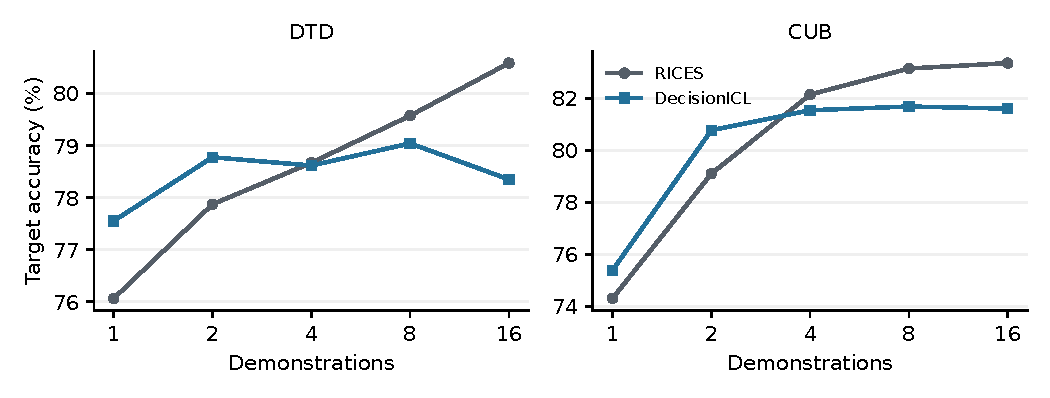
\includegraphics[width=.86\textwidth]{figures/shot_curve.pdf}
\caption{Exploratory accuracy under a fixed class selector as the demonstration budget increases. The first two points are main results with their budget-specific calibration. At four, eight, and sixteen demonstrations, the extension retains the two-shot coefficient and retrieves more examples within that selected class.}
\end{figure*}

\begin{table*}[t]
\caption{Complete larger-context results. Rescue, harm, and differences are oriented as \method minus RICES. Exact $p$ values are raw.}
\label{sup:shot_curve}
\centering\small
\begin{tabular}{llrrrrrr}
\toprule
Dataset & $k$ & RICES & +D & $\Delta$ & Rescue & Harm & Exact $p$ \\
\midrule
DTD & 4 & 78.67 & 78.62 & -0.05 & 77 & 78 & 1 \\
DTD & 8 & 79.57 & 79.04 & -0.53 & 79 & 89 & 0.488 \\
DTD & 16 & 80.59 & 78.35 & -2.23 & 65 & 107 & 0.00169 \\
CUB & 4 & 82.14 & 81.54 & -0.60 & 202 & 231 & 0.178 \\
CUB & 8 & 83.15 & 81.69 & -1.46 & 206 & 276 & 0.00165 \\
CUB & 16 & 83.35 & 81.60 & -1.75 & 213 & 297 & 0.000231 \\
\bottomrule
\end{tabular}
\end{table*}

At four demonstrations, the difference is $-0.05$ pp on DTD and $-0.60$ pp on CUB. At sixteen, the differences are $-2.23$ and $-1.75$ pp. The extension's selected class stays fixed as more examples are added. RICES can incorporate examples from additional classes. These outcomes describe expanding the prompt under the two-shot selector. Evaluation of a newly calibrated higher-budget method would require its own train/validation fit.

\section{Generic Direct-Sample Retrieval}
The Generic direct-sample alternative is a separate procedure that scores individual candidates with generic visual factors. It uses generic visual factor evidence to compare the query directly with each candidate training image. It fuses this evidence with the base's sample-level score and ranks the complete pool. Each dataset, budget, and base receives independent validation calibration. This alternative changes the retrieval structure as well as the factor source. The source-matched experiment in Appendix~\ref{sec:source} keeps the class-prototype structure fixed.

\begin{table*}[t]
\caption{Generic direct-sample comparison across all 25 Qwen3-VL-4B settings. The final column is Generic accuracy minus \method accuracy in percentage points.}
\label{sup:generic_direct}
\centering\small
\begin{tabular}{lllrrr}
\toprule
Dataset & $k$ & Base & Generic & DecisionICL & Generic minus D \\
\midrule
DTD & 1 & RICES & 76.97 & 77.55 & -0.59 \\
DTD & 1 & MUIER & 76.65 & 77.55 & -0.90 \\
DTD & 2 & RICES & 78.51 & 78.78 & -0.27 \\
DTD & 2 & MUIER & 78.40 & 79.04 & -0.64 \\
DTD & 2 & CIRCLES & 77.13 & 78.99 & -1.86 \\
Aircraft & 1 & RICES & 61.30 & 65.38 & -4.08 \\
Aircraft & 1 & MUIER & 62.53 & 64.75 & -2.22 \\
Aircraft & 2 & RICES & 63.85 & 65.71 & -1.86 \\
Aircraft & 2 & MUIER & 63.76 & 65.26 & -1.50 \\
Aircraft & 2 & CIRCLES & 61.63 & 65.56 & -3.93 \\
CUB & 1 & RICES & 74.28 & 75.39 & -1.11 \\
CUB & 1 & MUIER & 71.01 & 71.90 & -0.90 \\
CUB & 2 & RICES & 79.08 & 80.77 & -1.69 \\
CUB & 2 & MUIER & 75.51 & 76.43 & -0.92 \\
CUB & 2 & CIRCLES & 72.97 & 77.05 & -4.09 \\
Dogs & 1 & RICES & 72.86 & 74.37 & -1.52 \\
Dogs & 1 & MUIER & 76.48 & 76.77 & -0.29 \\
Dogs & 2 & RICES & 77.21 & 78.24 & -1.03 \\
Dogs & 2 & MUIER & 81.42 & 81.56 & -0.14 \\
Dogs & 2 & CIRCLES & 72.37 & 74.94 & -2.58 \\
Flowers & 1 & RICES & 92.99 & 93.15 & -0.16 \\
Flowers & 1 & MUIER & 92.26 & 92.75 & -0.49 \\
Flowers & 2 & RICES & 97.77 & 97.28 & +0.49 \\
Flowers & 2 & MUIER & 96.52 & 96.67 & -0.15 \\
Flowers & 2 & CIRCLES & 94.54 & 96.05 & -1.51 \\
\bottomrule
\end{tabular}
\end{table*}

Table~\ref{sup:generic_direct} shows that Generic direct-sample retrieval is below \method in 24 of the 25 settings, with an equal-setting mean difference of $-1.36$ points. Its best relative outcome is two-shot RICES on Flowers. The table compares complete retrieval procedures, while the matched-source table evaluates the narrower effect of discovery source under a common architecture.


\section{Additional Retrieval Baselines}
\label{sup:additional}
These completed single-run experiments extend the range of context-construction procedures. Their adapted prompts and retrieval features define separate panels from the main table. Tables~\ref{sup:vicl_accuracy} and~\ref{sup:promptself_accuracy} report every accepted dataset, budget, and source variant. Here +D denotes DecisionICL and +G denotes the Generic direct-sample variant. Each added selector receives its own train/validation calibration for the exact model, budget, and retrieval rule.

\paragraph{VICL task adaptation.}
VICL~\cite{vicl} uses visual demonstration retrieval, intent-oriented image summarization, and text-based demonstration composition. Our full-pool adaptation ranks training images by CLIP compatibility with a query description generated by the target VLM. Selected training images and their known labels produce task-oriented summaries. The final prompt contains the summaries and labels together with the query image. At two shots it contains two distinct training summaries. The base, DecisionICL, and Generic variants share this composition within each target and budget. The procedure changes both retrieval and demonstration representation relative to the ordinary image-example prompt, so its results form a separate protocol panel.

\begin{table*}[t]
\caption{Complete VICL full-pool task-adaptation accuracy. All entries are accepted single-run accuracies in percent. The full target name and precision identify each panel. The five-dataset mean is unweighted. +D and +G use the same summary-based target prompt as VICL.}
\label{sup:vicl_accuracy}
\centering\small\setlength{\tabcolsep}{6pt}
\begin{tabular}{llrrrrrr}
\toprule
$k$ & Method & DTD & Aircraft & CUB & Dogs & Flowers 102 & Mean \\
\midrule
\multicolumn{8}{l}{\textbf{Qwen3-VL-4B-Instruct (BF16)}} \\
1 & VICL & 68.30 & 40.11 & 37.21 & 58.69 & 82.75 & 57.41 \\
1 & VICL+D & 71.76 & 50.98 & 46.83 & 63.78 & 89.20 & 64.51 \\
1 & VICL+G & 70.90 & 50.53 & 52.25 & 62.63 & 89.07 & 65.08 \\
\addlinespace[2pt]
2 & VICL & 69.95 & 42.09 & 38.49 & 60.61 & 87.48 & 59.72 \\
2 & VICL+D & 74.52 & 58.30 & 52.19 & 66.81 & 94.78 & 69.32 \\
2 & VICL+G & 72.66 & 55.27 & 57.66 & 65.15 & 92.88 & 68.72 \\
\midrule
\multicolumn{8}{l}{\textbf{Qwen2.5-VL-7B-Instruct (NF4)}} \\
1 & VICL & 66.01 & 48.30 & 45.66 & 58.45 & 83.66 & 60.42 \\
1 & VICL+D & 73.14 & 59.56 & 62.58 & 68.04 & 91.61 & 70.98 \\
1 & VICL+G & 73.83 & 56.35 & 57.88 & 67.54 & 91.04 & 69.33 \\
\addlinespace[2pt]
2 & VICL & 69.79 & 49.08 & 49.19 & 60.96 & 86.58 & 63.12 \\
2 & VICL+D & 74.04 & 61.63 & 67.73 & 69.37 & 93.35 & 73.22 \\
2 & VICL+G & 75.43 & 59.92 & 63.29 & 71.07 & 93.64 & 72.67 \\
\bottomrule
\end{tabular}
\end{table*}

\paragraph{Prompt-SelF spatial-retrieval adaptation.}
The prompt-selection component of Prompt-SelF~\cite{promptself} compares spatial image features. Our classification adaptation uses frozen CLIP ViT-L/14 final-layer patch tokens at a $16\times16$ grid. We normalize each patch along its channels and average query-candidate cosine similarity over corresponding grid positions. Ranking covers the complete training pool. The target prompt remains the ordinary image-demonstration classification prompt. This experiment evaluates the retrieval component with a generative VLM and does not reproduce the original segmentation/detection system or its layout ensemble. Historical cache reuse preserves exact prompt identity, while the original record flags contexts whose batch partners may differ. These execution records remain separate from the main matrix.

\begin{table*}[t]
\caption{Complete Prompt-SelF spatial-retrieval adaptation with Qwen3-VL-4B-Instruct BF16. All entries are single-run accuracies in percent. +D uses class-prototype selection and +G uses direct-sample Generic evidence.}
\label{sup:promptself_accuracy}
\centering\small\setlength{\tabcolsep}{6pt}
\begin{tabular}{llrrrrrr}
\toprule
$k$ & Method & DTD & Aircraft & CUB & Dogs & Flowers 102 & Mean \\
\midrule
\multicolumn{8}{l}{\textbf{Qwen3-VL-4B-Instruct (BF16)}} \\
1 & Prompt-SelF & 63.83 & 41.94 & 34.33 & 58.62 & 77.46 & 55.24 \\
1 & Prompt-SelF+D & 72.45 & 59.17 & 50.25 & 67.25 & 90.45 & 67.91 \\
1 & Prompt-SelF+G & 71.76 & 56.56 & 61.06 & 66.01 & 90.54 & 69.18 \\
\addlinespace[2pt]
2 & Prompt-SelF & 66.60 & 44.46 & 37.32 & 62.21 & 82.92 & 58.70 \\
2 & Prompt-SelF+D & 73.67 & 59.47 & 52.63 & 69.83 & 94.47 & 70.01 \\
2 & Prompt-SelF+G & 75.90 & 58.93 & 66.10 & 69.44 & 95.48 & 73.17 \\
\bottomrule
\end{tabular}
\end{table*}

\paragraph{MMICES plan equivalence.}
MMICES~\cite{mmices} first retrieves visual candidates and then ranks their question text against the query question. In these classification tasks every question within a dataset is identical. With the frozen candidate budget of 128 and stable text ties preserving visual order, all 49,472 query-budget plans across the five datasets and two budgets match Qwen3-VL-4B RICES exactly. No separate target inference or extra accuracy row is needed for this question-only adaptation.

\paragraph{Paired statistics.}
Tables~\ref{sup:vicl_paired_qwen3}, \ref{sup:vicl_paired_qwen25}, and~\ref{sup:promptself_paired} give all source-variant comparisons with the matching adapted base. DecisionICL gains are positive in all 20 VICL settings and all 10 spatial-retrieval settings. Generic can be competitive with or exceed DecisionICL on individual datasets. These variants differ in both evidence source and class-versus-sample selection, so their contrast is separate from the matched-source control in Appendix~\ref{sec:source}.

\begin{table*}[t]
\caption{VICL paired comparisons with Qwen3-VL-4B-Instruct BF16. Each +D or +G row is compared with its VICL base. Differences and confidence intervals are in pp.}
\label{sup:vicl_paired_qwen3}
\centering\small\setlength{\tabcolsep}{6pt}
\begin{tabular}{lllrrrrr}
\toprule
Dataset & $k$ & Variant & Rescue & Harm & $\Delta$ (pp) & 95\% CI & Exact $p$ \\
\midrule
DTD & 1 & +G & 152 & 103 & +2.606 & [0.957, 4.309] & 0.00258 \\
DTD & 1 & +D & 105 & 40 & +3.457 & [2.234, 4.681] & 6.49e-08 \\
Aircraft & 1 & +G & 577 & 230 & +10.411 & [8.791, 12.031] & 3.41e-35 \\
Aircraft & 1 & +D & 514 & 152 & +10.861 & [9.391, 12.331] & 7.78e-47 \\
CUB & 1 & +G & 993 & 272 & +15.040 & [13.663, 16.479] & 1.11e-96 \\
CUB & 1 & +D & 692 & 231 & +9.616 & [8.406, 10.847] & 4.37e-54 \\
Dogs & 1 & +G & 791 & 453 & +3.939 & [3.124, 4.732] & 6.97e-22 \\
Dogs & 1 & +D & 686 & 250 & +5.082 & [4.382, 5.769] & 1.3e-47 \\
Flowers & 1 & +G & 505 & 116 & +6.326 & [5.546, 7.107] & 9.08e-59 \\
Flowers & 1 & +D & 418 & 21 & +6.456 & [5.806, 7.107] & 5.54e-97 \\
DTD & 2 & +G & 137 & 86 & +2.713 & [1.170, 4.309] & 0.000776 \\
DTD & 2 & +D & 151 & 65 & +4.574 & [3.032, 6.117] & 4.62e-09 \\
Aircraft & 2 & +G & 654 & 215 & +13.171 & [11.461, 14.851] & 3.31e-52 \\
Aircraft & 2 & +D & 744 & 204 & +16.202 & [14.461, 17.912] & 9.14e-73 \\
CUB & 2 & +G & 1123 & 204 & +19.170 & [17.772, 20.567] & 5.15e-154 \\
CUB & 2 & +D & 964 & 307 & +13.705 & [12.286, 15.102] & 2.77e-79 \\
Dogs & 2 & +G & 759 & 369 & +4.545 & [3.776, 5.303] & 1.25e-31 \\
Dogs & 2 & +D & 936 & 404 & +6.200 & [5.373, 7.028] & 5.87e-49 \\
Flowers & 2 & +G & 486 & 154 & +5.399 & [4.602, 6.196] & 5.55e-41 \\
Flowers & 2 & +D & 484 & 35 & +7.302 & [6.603, 7.985] & 4.04e-102 \\
\bottomrule
\end{tabular}
\end{table*}

\begin{table*}[t]
\caption{VICL paired comparisons with Qwen2.5-VL-7B-Instruct NF4. Each +D or +G row is compared with its VICL base. Exact $p$ values are two-sided McNemar values.}
\label{sup:vicl_paired_qwen25}
\centering\small\setlength{\tabcolsep}{6pt}
\begin{tabular}{lllrrrrr}
\toprule
Dataset & $k$ & Variant & Rescue & Harm & $\Delta$ (pp) & 95\% CI & Exact $p$ \\
\midrule
DTD & 1 & +G & 245 & 98 & +7.819 & [5.904, 9.734] & 1.16e-15 \\
DTD & 1 & +D & 201 & 67 & +7.128 & [5.479, 8.777] & 9.96e-17 \\
Aircraft & 1 & +G & 540 & 272 & +8.041 & [6.421, 9.691] & 3.18e-21 \\
Aircraft & 1 & +D & 593 & 218 & +11.251 & [9.661, 12.901] & 7.48e-41 \\
CUB & 1 & +G & 907 & 321 & +12.224 & [10.847, 13.600] & 4.33e-65 \\
CUB & 1 & +D & 999 & 188 & +16.917 & [15.603, 18.210] & 6.84e-134 \\
Dogs & 1 & +G & 1322 & 542 & +9.091 & [8.112, 10.047] & 5.41e-75 \\
Dogs & 1 & +D & 1224 & 401 & +9.592 & [8.695, 10.478] & 9.8e-97 \\
Flowers & 1 & +G & 527 & 73 & +7.383 & [6.635, 8.164] & 8.29e-86 \\
Flowers & 1 & +D & 510 & 21 & +7.953 & [7.221, 8.668] & 6.56e-123 \\
DTD & 2 & +G & 193 & 87 & +5.638 & [3.883, 7.394] & 2.15e-10 \\
DTD & 2 & +D & 176 & 96 & +4.255 & [2.553, 5.957] & 1.41e-06 \\
Aircraft & 2 & +G & 610 & 249 & +10.831 & [9.121, 12.481] & 1.03e-35 \\
Aircraft & 2 & +D & 674 & 256 & +12.541 & [10.801, 14.281] & 4.77e-44 \\
CUB & 2 & +G & 974 & 298 & +14.101 & [12.703, 15.499] & 5.07e-84 \\
CUB & 2 & +D & 1127 & 238 & +18.544 & [17.126, 19.942] & 1.84e-138 \\
Dogs & 2 & +G & 1385 & 517 & +10.117 & [9.161, 11.119] & 3.41e-91 \\
Dogs & 2 & +D & 1374 & 652 & +8.415 & [7.436, 9.429] & 5.48e-59 \\
Flowers & 2 & +G & 500 & 66 & +7.058 & [6.310, 7.790] & 1.64e-83 \\
Flowers & 2 & +D & 467 & 51 & +6.765 & [6.050, 7.481] & 3.57e-85 \\
\bottomrule
\end{tabular}
\end{table*}

\begin{table*}[t]
\caption{Prompt-SelF spatial-retrieval paired comparisons with Qwen3-VL-4B-Instruct BF16. Each +D or +G row is compared with its matching spatial-retrieval base. Exact $p$ values are raw.}
\label{sup:promptself_paired}
\centering\small\setlength{\tabcolsep}{6pt}
\begin{tabular}{lllrrrrr}
\toprule
Dataset & $k$ & Variant & Rescue & Harm & $\Delta$ (pp) & 95\% CI & Exact $p$ \\
\midrule
DTD & 1 & +G & 222 & 73 & +7.926 & [6.170, 9.734] & 1.21e-18 \\
DTD & 1 & +D & 222 & 60 & +8.617 & [6.915, 10.372] & 5.01e-23 \\
Aircraft & 1 & +G & 730 & 243 & +14.611 & [12.871, 16.382] & 3.55e-57 \\
Aircraft & 1 & +D & 712 & 138 & +17.222 & [15.602, 18.812] & 6.68e-94 \\
CUB & 1 & +G & 1507 & 226 & +26.721 & [25.198, 28.223] & 3.41e-232 \\
CUB & 1 & +D & 968 & 205 & +15.916 & [14.602, 17.251] & 6.79e-119 \\
Dogs & 1 & +G & 1077 & 443 & +7.389 & [6.527, 8.263] & 4.64e-61 \\
Dogs & 1 & +D & 989 & 249 & +8.625 & [7.867, 9.406] & 1.23e-104 \\
Flowers & 1 & +G & 870 & 66 & +13.075 & [12.165, 13.986] & 8.32e-180 \\
Flowers & 1 & +D & 832 & 33 & +12.994 & [12.116, 13.872] & 4.39e-201 \\
DTD & 2 & +G & 255 & 80 & +9.309 & [7.447, 11.170] & 2e-22 \\
DTD & 2 & +D & 213 & 80 & +7.074 & [5.266, 8.883] & 4.15e-15 \\
Aircraft & 2 & +G & 710 & 228 & +14.461 & [12.721, 16.172] & 3.22e-58 \\
Aircraft & 2 & +D & 691 & 191 & +15.002 & [13.291, 16.622] & 3.91e-67 \\
CUB & 2 & +G & 1598 & 218 & +28.786 & [27.201, 30.288] & 4.06e-259 \\
CUB & 2 & +D & 1020 & 286 & +15.311 & [13.913, 16.729] & 7.14e-97 \\
Dogs & 2 & +G & 1131 & 511 & +7.226 & [6.317, 8.147] & 5.9e-54 \\
Dogs & 2 & +D & 1095 & 442 & +7.611 & [6.725, 8.497] & 4.74e-64 \\
Flowers & 2 & +G & 833 & 61 & +12.555 & [11.660, 13.466] & 4.26e-174 \\
Flowers & 2 & +D & 768 & 58 & +11.547 & [10.668, 12.409] & 4.05e-159 \\
\bottomrule
\end{tabular}
\end{table*}

\section{Reproduction and Evidence Records}
\paragraph{Bank construction.}
The target VLM receives training images and the task's class names. Structured responses contain a reusable visual property, its states, and state descriptions. The discovery requests use complementary appearance perspectives. Format checks, duplicate handling, and the corresponding frozen evidence-processing protocol produce the retained bank. Qwen2.5-VL-7B and Gemma use their separately recorded discovery requests and responses. The Qwen3-VL-4B main table retains its accepted task-specific banks. The source-matched controls in Appendix~\ref{sec:source} use their own matched discovery budgets, so they are reported separately from the main-table banks.

\paragraph{Distribution agreement.}
For probability vectors $u$ and $v$, let $m=(u+v)/2$. The Jensen-Shannon divergence used in the main paper is
\begin{equation}
\begin{split}
\operatorname{JSD}(u,v)={}&\tfrac12\sum_s u_s\log\frac{u_s}{m_s}\\
&+\tfrac12\sum_s v_s\log\frac{v_s}{m_s}.
\end{split}
\end{equation}
The index $s$ runs over a factor's states. Zero-probability terms contribute zero. Natural logarithms give a maximum of $\log 2$, which supplies the normalization in the agreement score. This score compares whole-image factor evidence with a training-class prototype.

\paragraph{Calibration.}
The mixture-coefficient grid is $\{0,0.05,0.1,0.2,0.35,0.5,0.65,0.8,1\}$. Equal validation scores prefer larger base weight. The fit applies to one exact target and dataset. It is repeated independently for every budget and base under the corresponding factor-bank and evidence contract. Decision factors share the remaining weight equally. The final full-validation fit supplies the coefficient for test class selection. Out-of-fold fits characterize calibration behavior without changing the final retrieval rule.

\paragraph{Frozen execution contract.}
Each accepted block binds the data manifests and factor bank. It also records visual evidence and calibration. The ordered demonstration plan is linked to the target model's prompt and decoding configuration. Final VLM answers retain their raw generated text. Complete and independent-audit receipts identify the files behind each result. Repeated runs additionally bind exported work orders to imported target outputs.

\paragraph{Fixed batching.}
Contexts are deduplicated only when their complete prompt identity agrees. Two-context execution fixes the partner context as part of the inference record. The accepted historical Qwen3-VL-4B DTD one-shot block uses single-context execution. Original and resumed outputs retain the same fixed-group contract. The repeat roots preserve separate seed-specific logs and preparation receipts. These details allow raw output, context identity, and final method-query VLM answers to be checked together.

\paragraph{Execution variation in the class-selection ablation.}
Factor-informed and base-class selection produce identical ordered demonstrations for 1,671 DTD queries, 2,329 Aircraft queries, and 4,495 CUB queries. Final VLM answers differ on 5 DTD queries. They differ on 13 Aircraft queries and 14 CUB queries with identical ordered demonstrations. Each method follows its fixed batch protocol, so batch partners can differ across the two experiments. We retain these outcomes in all reported paired results. The retrieval changes and the final target outcomes are recorded separately in the evidence files.

\paragraph{Result construction.}
The main matrix contains 180 method results and 75 base-versus-DecisionICL comparisons. Additional published controls contain 25 Generic direct-sample results and three results each for base-class selection, prototype rotation, and visual-centroid selection. The matched-source experiment has four source comparisons. The auxiliary VICL and Prompt-SelF panels contain 90 additional single-run method results and 60 paired variant comparisons. The two new Qwen3-VL-4B runs contain 120 additional method results, and the larger-shot study contains twelve additional method results. These groups are kept separate in the reported tables.

\paragraph{Computation structure.}
Let $N$ be the number of training images and $C$ the number of classes. The base embedding dimension is $d$. The total number of factor states is $S=\sum_gS_g$. Training-state evidence and class prototypes are precomputed. A query with one base ranking computes training-pool similarities at cost proportional to $Nd$. State-text similarities cost the evidence embedding dimension times $S$. Query-class distribution agreement costs $CS$. Class selection takes the argmax of the fused scores. It returns the index of the training class used for retrieval. The final target VLM context still contains one or two demonstrations. Factor discovery is performed offline for each target and dataset.

\paragraph{Figures and qualitative examples.}
The Aircraft traces follow the example rule in Appendix~\ref{sup:traces}. Query and demonstration images are checked against their manifest hashes. Frozen mathematical functions replay state-distribution agreement and score standardization on the CPU. The displayed values and selected images come from these records. Final VLM answers are retained from the accepted inference outputs. The figures place those answers after demonstration retrieval.

{\small
\bibliographystyle{ieeenat_fullname}
\bibliography{references}
}
\end{document}
